\documentclass[12pt,a4paper]{article}
\usepackage[utf8]{utf8}
\usepackage[margin=1in]{geometry}
\usepackage{tcolorbox}
\usepackage{tikz}
\usetikzlibrary{shapes.geometric, arrows.meta, positioning}

\title{\textbf{Childhood}\\[0.3em] \Large Textbook Page 43}
\author{\textbf{Poet:} Markus Natten \quad|\quad \textbf{Textbook:} Hornbill (Class 11)}
\date{}

\begin{document}

\maketitle

\section*{Text Content}

\begin{verse}
When did my childhood go?\\
Was it the day I ceased to be eleven,\\
Was it the time I realised that Hell and Heaven,\\
Could not be found in Geography,\\
And therefore could not be,\\
Was that the day!\\
\end{verse}

\vspace{0.5cm}

\begin{verse}
When did my childhood go?\\
Was it the time I realised that adults were not\\
all they seemed to be,\\
They talked of love and preached of love,\\
But did not act so lovingly,\\
Was that the day!\\
\end{verse}

\vspace{0.5cm}

\begin{verse}
When did my childhood go?\\
Was it when I found my mind was really mine,\\
To use whichever way I choose,\\
Producing thoughts that were not those of other people\\
But my own, and mine alone\\
Was that the day!\\
\end{verse}

\vspace{0.5cm}

\begin{verse}
Where did my childhood go?\\
It went to some forgotten place,\\
That's hidden in an infant's face,\\
That's all I know.\\
\end{verse}

\vspace{1cm}

\begin{figure}[htbp]
\centering
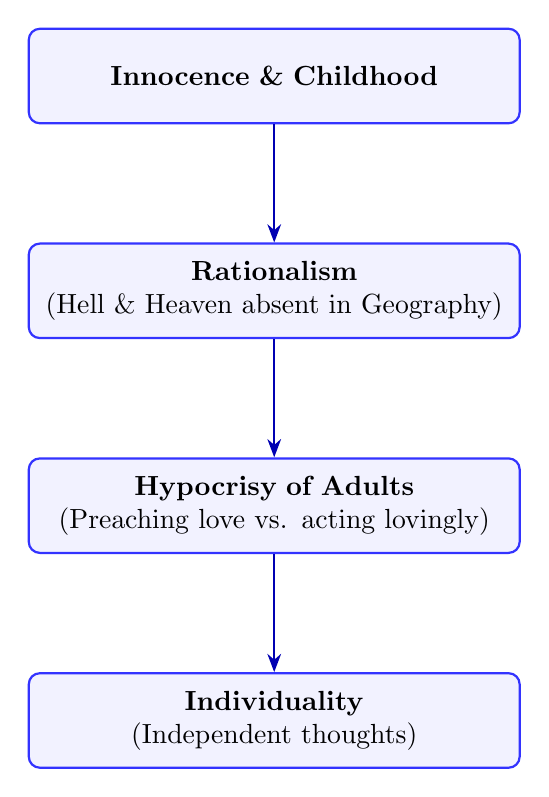
\begin{tikzpicture}[
    node distance=1.5cm,
    block/.style={rectangle, draw=blue!80, fill=blue!5, thick, rounded corners, text width=6cm, align=center, minimum height=1.2cm},
    arrow/.style={-Stealth, thick, draw=blue!70!black}
]
    \node[block] (innocence) {\textbf{Innocence \& Childhood}};
    \node[block, below=of innocence] (rational) {\textbf{Rationalism}\\ (Hell \& Heaven absent in Geography)};
    \node[block, below=of rational] (hypocrisy) {\textbf{Hypocrisy of Adults}\\ (Preaching love vs. acting lovingly)};
    \node[block, below=of hypocrisy] (individuality) {\textbf{Individuality}\\ (Independent thoughts)};

    \draw[arrow] (innocence) -- (rational);
    \draw[arrow] (rational) -- (hypocrisy);
    \draw[arrow] (hypocrisy) -- (individuality);
\end{tikzpicture}
\caption{Page 43: Transition Stages of Growing Up in \textit{Childhood}}
\end{figure}

\end{document}
\documentclass[12pt,a4paper]{article}
\usepackage[utf8]{utf8}
\usepackage[margin=1in]{geometry}
\usepackage{tcolorbox}
\usepackage{tikz}
\usetikzlibrary{shapes.geometric, arrows.meta, positioning}

\title{\textbf{Childhood — Exercises}\\[0.3em] \Large Textbook Page 44}
\author{\textbf{Poet:} Markus Natten \quad|\quad \textbf{Textbook:} Hornbill (Class 11)}
\date{}

\begin{document}

\maketitle

\section*{Think It Out}

\begin{enumerate}
    \item Identify the stanza that talks of each of the following:
    \begin{itemize}
        \item individuality
        \item rationalism
        \item hypocrisy
    \end{itemize}
    \item What according to the poem is involved in the process of growing up?
    \item What is the poet's feeling towards childhood?
    \item Which do you think are the most poetic lines? Why?
\end{enumerate}

\section*{Understanding the Poem}
Questions are based on:
\begin{itemize}
    \item Thematic comprehension
    \item Reflection on theme
    \item Poetic sensibility
\end{itemize}

\vspace{1cm}

\begin{figure}[htbp]
\centering
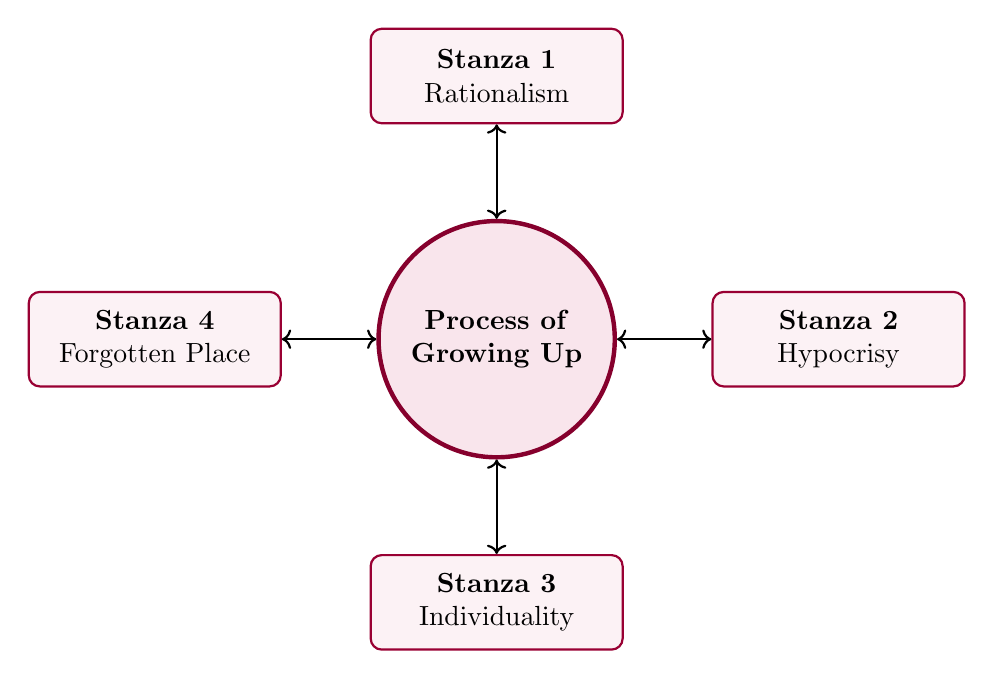
\begin{tikzpicture}[
    center/.style={circle, draw=purple!70!black, fill=purple!10, ultra thick, minimum size=3cm, align=center},
    theme/.style={rectangle, draw=purple!80!black, fill=purple!5, thick, rounded corners, minimum width=3.2cm, minimum height=1.2cm, align=center}
]
    \node[center] (core) {\textbf{Process of}\\ \textbf{Growing Up}};
    \node[theme, above=1.2cm of core] (rat) {\textbf{Stanza 1}\\ Rationalism};
    \node[theme, right=1.2cm of core] (hyp) {\textbf{Stanza 2}\\ Hypocrisy};
    \node[theme, below=1.2cm of core] (ind) {\textbf{Stanza 3}\\ Individuality};
    \node[theme, left=1.2cm of core] (lost) {\textbf{Stanza 4}\\ Forgotten Place};

    \draw[<->, thick] (core) -- (rat);
    \draw[<->, thick] (core) -- (hyp);
    \draw[<->, thick] (core) -- (ind);
    \draw[<->, thick] (core) -- (lost);
\end{tikzpicture}
\caption{Page 44: Analytical Map of Exercises and Stanza Themes}
\end{figure}

\end{document}

